\subsubsection{Two-dimensional array example}

We are going to work with an array of type \Tchar, which implies that each element requires only one 
byte in memory.

\myparagraph{Row filling example}
\myindex{\olly}

Let's fill the second row with these values 0..3:

\lstinputlisting[caption=Row filling example,style=customc]{patterns/13_arrays/5_multidimensional/two1_EN.c}

All three rows are marked with red. 
We see that second row now has values 0, 1, 2 and 3:

\begin{figure}[H]
\centering
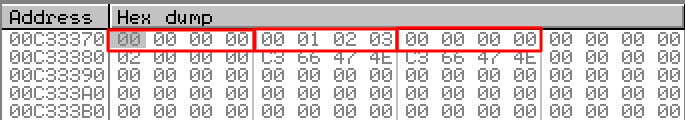
\includegraphics[width=0.6\textwidth]{patterns/13_arrays/5_multidimensional/olly_2D_1.png}
\caption{\olly: array is filled}
\end{figure}

\myparagraph{Column filling example}
\myindex{\olly}

Let's fill the third column with values: 0..2:

\lstinputlisting[caption=Column filling example,style=customc]{patterns/13_arrays/5_multidimensional/two2_EN.c}

The three rows are also marked in red here. 

We see that in each row, at third position these values are written: 0, 1 and 2.

\begin{figure}[H]
\centering
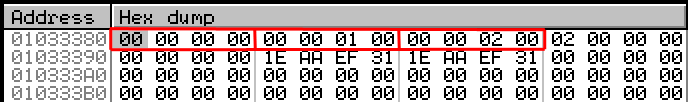
\includegraphics[width=0.6\textwidth]{patterns/13_arrays/5_multidimensional/olly_2D_2.png}
\caption{\olly: array is filled}
\end{figure}

